\chapter{Numerical Methods}
\section{The Finite Element Method}
The theory presented in this section is partly inspired by the works of Langtangen in "Finite Element Method - INF5620 lecture notes" \cite{Lang2}  \\
Consider the Poisson-equation
\begin{align}
-\nabla^2 v = f & \quad \text{ in } \Omega \label{Poisson}\\
v = v_0 & \quad \text{ on } \partial \label{Poisson_D}\Omega_D \\
\pdi{v}{n} = g & \quad \text{ on } \partial \Omega_N \label{Poisson_N}
\end{align}
where $\Omega \in \mathbb{R}^d$ is a domain, $ v = v(x)$ is an unknown function and $f$ is a source function. The boundary, $\partial \Omega$ is divided into two parts. $\partial \Omega_D$ for the Dirichlet boundary condition, and $\partial \Omega_N$ for the Neumann condition. 
\\
\\
\subsection{Variational formulation}
\eqref{Poisson} is known as the strong form of the equation. To reformulate the problem and state a weak formulation we multiply the equation with a test function, $\phi \in \hat{V}$, where $\hat{V}$ is some function space, and integrate over the domain. Weak formulations are important in the sense that differential equations can be transformed into systems of linear equations. In the rest of this text the following notation is used for the inner product of two functions
\begin{align} (v,\phi)_{\Omega} = \int_{\Omega} v \, \phi \, \mathrm{d}x
\end{align}

By multiplying \eqref{Poisson} with a test function, $\phi$ and integrating over the domain, the weak form is obtained
\begin{align}
(\nabla^2 v + f, \phi)_\Omega = 0 & \quad \forall \, \phi \in\hat{V} \label{Projection}
\end{align}
We are now searching for a $v$ to satisfy the weak form instead of the strong. T
This equation should hold for all $\phi$ in the function space $\hat{V}$. The trial function does not necessarily have to lie in the same function space, in general $v \in V$. \\

 In this thesis we will use two Sobolov spaces (named after the Russian mathematician Sergei Sobolov) widely used in Finite Element computing. For these definitions to be valid, we assume that the functions $v$ are all \textbf{|locally integrable} and in the case of definition \eqref{H1}, has one \textbf{weak derivative}. For more details on weak derivatives and the generalized concept of Sobolev spaces and functional analysis, we refer to the textbook by Brenner and Scott \cite{Bren07}.   
\begin{definition}
Let $\Omega$ be an open subset of $\mathbb{R}$ with a piecewise smooth boundary. We then define the $L^2$-norm as follows\\ \begin{center}
$||v||_{L^2(\Omega)} = (\int_\Omega v^2 \mathrm{d}x)^{\frac{1}{2}}$
\end{center}
The corresponding $L^2$-space is defined via
\begin{center}
$L^2(\Omega) = \{ v:\Omega \rightarrow \mathbb{R} | \int_\Omega v^2 \mathrm{d}x < \infty \}$
\end{center}
\label{|l2}
\end{definition}
\begin{definition}
Let $\Omega$ be an open subset of $\mathbb{R}$ with a piecewise smooth boundary. We then define the $H^1$-norm as follows\\ \begin{center}
$||v||_{H^1(\Omega)} = (\int_\Omega [v^2 + (\nabla v)^2]\mathrm{d}x)^{\frac{1}{2}}$
\end{center}
The corresponding $H^1$-space is defined via
\begin{center} $H^1(\Omega) = \{ v:\Omega \rightarrow \mathbb{R} | \int_\Omega [v^2 + (\nabla v)^2] \mathrm{d}x < \infty \}$
\end{center}
\label{H1}
\end{definition}
In other words, using functions from these spaces, we can have some assurance that the integrals involved in the variational form are bounded. 
By the divergence theorem, a generalized concept of integration by parts we can state the variational problem as follows: find $v \in V$ such that \\ \\
\begin{align}
(\nabla v, \nabla \phi)_\Omega = (f,\phi)_\Omega + (g, \phi)_{\partial \Omega_N}& \quad \forall \, \phi \in \hat{V} \label{Weak_form}
\end{align}
\\
Where we have used that $\pdi{v}{n} = g$ on $\partial \Omega_N$. \eqref{Weak_form} is known as the variational formulation of the Poisson problem.  The left hand side is known as the bilinear form while the right hand side is the linear form. In generic form the equation can be written
\begin{align}
a(v,\phi) = L(\phi) \label{Bilinear}
\end{align}
The first derivative of $v$ appears in the variational form. A common choice is then
\begin{align}
 V := \{ v \in H^1(\Omega) : v = v_0 \text{ on } \partial \Omega_D \} \\
 \hat{V} := \{ v \in H^1(\Omega) : v = 0 \text{ on } \partial \Omega_D \}
\end{align}
In other words, the trial and test functions are in the same function space, except on the boundary.



\subsection{Finite elements} \label{FinEle}
The next step is to approximate $v$ with a sum of basisfunctions in the finite-dimensional function space, $V = \text{span}\{\phi_0, \phi_1, ..., \phi_N \}$. Here, $\phi_i$ represents the basis functions and we search for a solution $v_h \in V$ such that $v_h$ can be written as a linear combination of the basis functions. 
The first step in the finite element method consists of dividing the domain into smaller parts
\begin{align*}
\Omega = \Omega_0 \cup \Omega_1 \cup ... \cup \Omega_{N_e}
\end{align*}
where $N_e$ is the number of elements. Each element have a number of nodes within them depending on what type of basis functions to be used. Let's first consider the continuous Galerkin basis functions, in a one-dimensional domain. There is exactly one basisfunction for each node located at $x_i$. These basis functions have the property that
\begin{align*}
\phi_i(x_j) = \begin{cases}
				1 \quad \text{ for } i=j \\
				0 \quad \text{ for } i\neq j
		 		\end{cases}
\end{align*}
\begin{figure}[!ht]
  \begin{center}
    \includegraphics[scale=0.4]{figures/hats.png}
  \end{center}
	\caption{The three first linear basis functions on the unit interval divided uniformly into 5 elements, $\Omega_0 = [0,0.2], \Omega_1 = [0.2,0.4]$ and so on. In the case of Dirichlet Boundary conditions at $x=0$, $\phi_0$ will not be included in the funtcion space}
	\label{fig:Hats}
\end{figure}
\\
That is, the basis functions $\phi_i$ are zero on all nodes except at node $i$. Each basis function is constructed by taking the Lagrange-polynomial which is 1 at the given node and 0 on the neighboring nodes. Note that the basis functions are two Lagrange-polynomials "pieced together" at the node where it's value is 1. For the rest of the domain the basis functions are defined to be 0. \\ \\

Now, let's return to the original problem \eqref{Poisson}-\eqref{Poisson_N} in scalar form. We start by approximating $v$ as a linear combination of all the basis functions. 
\begin{align}
v_h = \sum_{i=0}^N c_i \phi_i \label{u_hsum}
\end{align}
The definitions of $v_h$ and $V$ now give rise to a linear system. Using the Einstein summation convention, $x_i\,y_i = \sum_0^N x_i y_i $, the discretized version of \eqref{Weak_form} is now written 
\begin{align}
-c_i(\nabla \phi_i, \nabla \phi_j)_\Omega = (f,\phi_j)_\Omega - (g, \phi_j)_{\partial \Omega_N} \label{|linear_system}
\end{align}
\\
\\

In the case of Dirichlet boundary conditions all test functions $\phi_j$ will take the value 0 on $\partial \Omega_D$ and the linear system will be adjusted to take these boundary conditions into account. \\
The system can be written in matrix form, and in the end the problem consists of solving the linear system
\begin{align} A_{i,j}c_i = b_j \label{Matrix_1} \end{align}
\\
\\
\section{The FEniCS software} 
When the variational form has been carried out, implementation in FEniCS is relatively simple. The programs in this study are written in the Python programming language. When programming with Python, we first need to import dolfin to access the DOLFIN library, containing classes convinient and efficient for finite element computing. In Python the full library can be imported as simple as 
\begin{verbatim}
from dolfin import *
\end{verbatim}
Now, let's focus our attention on solving the following problem:
\begin{align}
\nabla^2v = 20x \,\,\,\,\, \text{ in } \Omega \\
v(0,y) = 0, \,\,\,\, v(1,y) = 1 \\
\pdi{v(x,0)}{n} = \pdi{v(x,1)}{n} = 0
\end{align}
Where $\Omega$ is the unit square, $\Omega = [0,1] \times [0,1]$ \\
\\
First of all we need to define the computational mesh.
\begin{cverbatim}
mesh = UnitSquareMesh(10,10)
\end{cverbatim}
The class UnitSquareMesh initializes a mesh with triangular cells. The mesh consists of n$\times$m squares depending on the arguments, $n$ and $m$, sent into the constructor. Each of these squares are divided on the diagonal to form two triangles, and these triangles are the computational cells. In this case we get the unit square divided into 10$\times$10 smaller squares and thus the total number of triangles, or cells, will be 200. \\
The next thing to do is to define an appropriate function space for the test functions. The solution will be a linear combination of these functions and will be in (almost) the same function space. 
\begin{cverbatim}
V = FunctionSpace(mesh,'CG',1)
\end{cverbatim}
The function space needs a domain, type of element, and the degree of the element. In this case we use Continuous Galerkin elements ('CG') with degree 1. These basis functions are visualized in Figure \ref{fig:Hats}
\\ We can then define our test- and trial functions $v$ and $\phi$
\begin{cverbatim}
v = TrialFunction(V)
phi = TestFunction(V)
\end{cverbatim}
Note that the test- and trial function seem to be in the exact same function space. This is the case except when imposing Dirichlet boundary conditions. 
The functions $f$, $v_0$ and $g$ can be defined by using the 'Constant' or 'Expression' classes. We set $f = 20x$ and use Dirichlet boundary conditions, $v(0,y) = 0$, $v(1,y) = 1$ and Neumann conditions $\pdi{v(x,0)}{n} = \pdi{v(x,1)}{n} = 0$. The homogenuous Neumann condition is simple in the finite element method as the terms appearing after integration by parts can be dropped. If this is not the case, we can insert $g$ for $\pdi{u}{n}$ on the boundary integral appearing in the variational form. When the Neumann conditions are incorporated this way we say that the boundary conditions are weakly imposed. Functions (or classes) describing the boundaries must also be defined:
\begin{cverbatim}
f = Expression('20*x[0]')
def boundary0(x,on_bnd):
	return on_bnd and near(x[0],0.0)
def boundary1(x,on_bnd):
	return on_bnd and near(x[0],1.0)

bc0 = DirichletBC(V,0.0,boundary0)
bc1 = DirichletBC(V,1.0,boundary1)
bcs = [bc0,bc1]
\end{cverbatim}
Note that 'x[0]' means first dimension in space, 'x[1]' means second dimension and so on. The Dirichlet conditions are put in a list. Next, the variational form is defined, and when solving for a function v, the boundary conditions are added to the "magic" solve function. 
\begin{cverbatim}
F = inner(grad(v),grad(phi))*dx - inner(f,phi)*dx
v = Function(V)
solve(lhs(F)==rhs(F),v,bcs)
plot(v)
\end{cverbatim}
The functions lhs and rhs separates the form F into the left hand side, equivalent to the bilinear form and to the right hand side, equivalent to the linear form. Specifying the full form F is simple and convenient when the equations are short and simple. If we want to relate the code to the mathematics as written in \eqref{Bilinear} we can, define these forms manually. 
\begin{cverbatim}
a = inner(grad(v),grad(phi))*dx
L = inner(f,phi)*dx
v = Function(V)
solve(a==L,v,bcs)
\end{cverbatim}
\begin{figure}[!h]
\includegraphics[scale=0.5]{figures/poisson_f_20x}
\caption{Plot of the computed solution}
\end{figure}
The plot in the figure is slightly rotated. The solution is independent of y-position, as expected. 	

\section{A Discontinuous Galerkin method}
Discontinuous Galerkin (DG) methods is a relatively new tool for CFD simulations. The method itself was developed during the 1970s and has been used increasingly the last few decades. Unlike with the Continuous Galerkin elements, we now allow the solution to be discontiuous, i.e cells do not share nodes anymore. Instead of solving over the whole domain, we now seek approximate continuous solutions on each cell independently of the others. To this end it is convenient to define the average and jump of a discontinuous variable
\begin{align} 
\{\mathbf{v}\} = \frac{1}{2}(\mathbf{v}^+ + \mathbf{v}^-) \hspace{2 cm}  [\mathbf{v}]  =  \mathbf{v}^+ - \mathbf{v}^- \label{Avg_jump}
\end{align}
where $\mathbf{v}^+$ and $\mathbf{v}^-$ is the solution at two neighboring cells at cell $E^+$ and $E^-$. These definitions can be accessed easily in FEniCS as
\begin{center}
\begin{cverbatim}
avg(v)
jump(v)
\end{cverbatim}
\end{center}
The normal vectors are denoted $\mathbf{n}^+$ and $\mathbf{n}^-$. If consistent, the choice of $\mathbf{n}$ is arbitrary. \cite{Rivi08}
\\
\\
It should be noted that \textit{the weak form presented here are not used in the spinal cord simulation in this thesis} as there were problems with the correct boundary conditions at the interface. The reason for including a short discussion about a DG-method lies in the advantage of having functions discontinuous over the interface between the fluid and the solid, escpecially in the Biot problem. For instance, if a function $\mathbf{v}$ should describe the fluid velocity in the fluid, and the structural velocity in the solid for the Biot problem, this variable would have to be discontinuous over the interface. FEniCS does not currently have the possibility to have discontinuous elements over the interface only, and therefore the function would have to be considered discontinuous over the whole domain.
\subsection{Stokes flow}
Consider the following problem in $\Omega = [0,1]\times[0,1]$:
\begin{align}
\nabla \cdot \sigma = 0 & \text{ in } \Omega \\
\nabla \cdot \mathbf{v} =  0 & \text{ in } \Omega\\
\mathbf{v} = 0 & \text{ on } \Omega_{\text{w}} \\
p \mathbf{n} - \mu \pdi{\mathbf{v}}{n} = p_{\text{in}}\mathbf{n} & \text{ on } \Omega_{\text{in}} \\
p \mathbf{n} - \mu \pdi{\mathbf{v}}{n} = p_{\text{out}}\mathbf{n} & \text{ on } \Omega_{\text{out}} \\
\end{align}
where $\sigma$ is the incompressible Newtonian fluid stress tensor as previously described. The inlet is at x=0, while the outlet is at x=1. The rigid walls are situated where y=0 and y=1. By choosing $p_{\text{in}} = 2$, $p_{\text{out}} = 0$, a steady Poiseuille flow should be obtained. The boundary condition on the inlet and outlet are Pseudo-traction as described in chapter 3. The equations describes what is often known as Stokes flow.  \\
By integrating Stokes equation by parts, adding symmetry and penalty terms as explained by Rivi{\`e}re and Yotov \cite{Rivi05} we end up with a consistent DG-method. Since the method involves many terms we derive the weak formulation term by term. The set of all elements are denoted as $e$, interior facets as $\Gamma$ and exterior facets as $\partial \Omega$. Starting with the diffusion term in divergence form, we multiply with a test function and integrate by parts:
\begin{align}
	2\mu \sum_{E \in e} (\epsilon(\mathbf{v}), \epsilon(\Phi))_E &
   -2\mu \sum_{E \in \Gamma}(\{\epsilon(\mathbf{v}) \} \cdot \mathbf{n}_e, [ \nabla \Phi ])_E 
   -2\mu \sum_{E \in \Gamma}(\{\epsilon(\mathbf{\Phi}) \} \cdot \mathbf{n}_e, [ \nabla \mathbf{v} ])_E \\
	& + \frac{\beta}{h} \sum_{E \in \Gamma}([\mathbf{v}],[\Phi])_E 
	-2\mu \sum_{E \in \partial \Omega}(\Phi,  \epsilon( \mathbf{v}) \cdot \mathbf{n}_e)_E \\
   & -2\mu \sum_{E \in \partial \Omega}(\mathbf{v},  \epsilon( \Phi)  \cdot \mathbf{n}_e)_E 
	+ \frac{\beta}{h} \sum_{E \in \partial \Omega}(\mathbf{v},\Phi)_E 
 \label {Diffusion}
\end{align}
Similiarly, the contributions from the term $-\nabla p$ will be
\begin{align}
	- \sum_{E \in e}(p, \nabla \cdot \Phi)_E + \sum_{E \in \Gamma}(\{p\},[\mathbf{\Phi}]\cdot \mathbf{n}) + \sum_{E \in \Gamma}(\{ \eta \},[\mathbf{v}]\cdot \mathbf{n})
\end{align}
With $DG_1\times DG_0$ elements for velocity and pressure the following results were obtained with the convergence rate computed as 
\begin{align}
\frac{\ln(\frac{e^{n+1}}{e^n})}{\ln(\frac{h^{n+1}}{h^n})},
\end{align}
N representing the number of cells in the $N\times N$ unit square and $h$ computed in FEniCS as mesh.hmin() for each refinement
\begin{table}[!h]
\begin{center}
  \begin{tabular}{|l | l | l | l| l| l|} \hline
	N & dofs & $||v-v_h||_{L^2}$&  $||p-p_h||_{L^2}$ & rate u & rate p\\ \hline
    4 & 224 & 1.8318e-02 & 1.5590e-01 & -- & --\\   \hline
    8 & 896 & 1.0732e-02 & 7.6566e-02 & 0.7713 & 1.0259 \\ \hline
    16 & 3584 & 5.8110e-03 & 3.7890e-02 & 0.8851 & 1.0149 \\ \hline
	32 & 14336 & 3.0221e-03 & 1.8895e-02 & 0.9432 & 1.0038 \\ \hline
	64 & 57344 & 1.5410e-03 & 9.4481e-03 & 0.9717 & 0.9999 \\ \hline
	128 & 229376 & 7.7808e-04 & 4.7267e-03 & 0.9859 & 0.9992 \\ \hline \hline
  \end{tabular}
\end{center}
\end{table}

\section{Womersley Flow}
In the cardiovascular system, pressure pulses travel along different blood vessels such as veins, capillaries and the aorta. These types of pulsating flows in tubes or channels have been given the name Womersley flow. The characteristics and velocity profile of the flow depends of several parameters such as the length of the tube or channel, pulsation frequency and fluid properties. In the end, the ratio between transient inertial forces and viscous forces is the fundamental difference separating flow patterns in pulsating flow. To this end the Womersley number, $\alpha$ is defined as follows:
\begin{align}
\alpha^2 = \frac{\text{transient intertial force}}{\text{viscous force}} = \frac{\rho\omega V}{\mu V L^{-2}} = \frac{L^2 \omega \rho}{\mu}
\end{align}
Where, $\rho$ is the fluid denisty, $\mu$ is the dynamic viscosity, $L$ is a length scale and $\omega$ is the pulsation frequency. In the 2D-model presented here, the modeling of SAS around the spinal cord consists of two channels where the Womersley number
\begin{align}
\alpha = L\big{(}\frac{\omega \rho}{\mu}\big{)}^{\frac{1}{2}},
\end{align}
would have a large impact on the flow characteristics. A low Womersley number (typically $\alpha < 1$ means the frequency is relatively low so the flow develops a velocity profile close to a parabola at each cycle. When $\alpha$ is large ($\alpha > 10$) the inertial forces dominate and more complicated phenomena such as bidirectional flow, i.e. flow in opposite directions over a cross section, could occur. 
\\
\\
Even though the flow should be aligned with the channel due to the incompressibility constraint, pulsating flow tends to give rise to some horizontal or radial flow with the boundary conditions previously described due to numerical errors. We will return to this issue in the next subsection. For now we assume the following conditions to hold 
\begin{align}
\mathbf{v}\cdot \tau = 0 & \text{ on } \partial \Omega_{\text{in}} \\
\mathbf{v}\cdot \tau = 0 & \text{ on } \partial \Omega_{\text{out}} \label{P_out}
\end{align}
Where $\tau$ is the tangential vector on the boundary surface.
\\
\\
The velocity and pressure should therefore satisfy
\begin{alignat}{4}
\pdi{\mathbf{v}}{t} + (\mathbf{v} \cdot \nabla ) \mathbf{v} & = \nabla \cdot \sigma \quad & \text{ in } \Omega, \\
\nabla \cdot \mathbf{u} & = 0 \quad & \text{ in } \Omega, \\
\mathbf{v} & =0 \quad & \text{ on } \Omega_{\text{w}}, \\
\mu \pdi{\mathbf{v}}{n} - p\mathbf{n} = p_{\text{in}}(t)\mathbf{n} & \text{ and } \mathbf{v}\cdot \tau  = 0 \quad & \text{ on } \Omega_{\text{in}}, \\
\mu \pdi{\mathbf{v}}{n} - p\mathbf{n} = p_{\text{out}}(t)\mathbf{n} & \text{ and } \mathbf{v}\cdot \tau = 0 \quad &  \text{ on } \Omega_{\text{out}}. \label{Womersley}
\end{alignat}
\\
\\
Exact solutions exists to both the channel and pipe cases. Langlois and Deville \cite{Lang64} have derived several solutions to equations of viscous flow, including channel flow with a pulsatile pressure gradient as above. We now add a oscillating pressure gradient so that
\begin{align}
-\frac{1}{\rho}\pdi{p}{x} = -C\cos(\omega t)
\end{align}
\begin{center}
\begin{figure}[!ht]
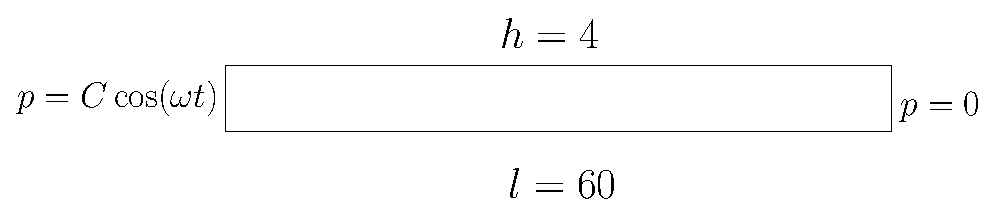
\includegraphics[width=\linewidth]{figures/Womersley}
\caption{Schematic of Womersley flow with dimensions as in the spinal cord} \label{fig:Wom}
\end{figure}
\end{center}

where C is a constant describing the strength of the pulse. Due to the assumption of axial flow only, the momentum equation in x-direction gives:
\begin{align}
\pdi{v_1}{t} = -\frac{1}{\rho}\pdi{p}{x_1} + \nu \pdi{^2v_1}{x_2^2} \label{NS_easy}
\end{align}
The presented solution did not correspond to the simulations at all, therefore an opportunity to utilize the symbolic python package sympy arised. The solution presented by Langlois and Deville was
\begin{align}
v_1 = -\frac{C}{\omega}\Bigg{[}\Big{(}1 - \frac{f_1(\omega,x_3)}{f_3(kh)}\Big{)}\sin(\omega t) - \frac{f_2(\omega,x_3)}{f_3(kh)}\cos(\omega t)\Bigg{]}
\end{align}
where
\begin{align}
k & = \sqrt{\frac{\omega}{2\nu}} \\
cc(x) & = \cos(x)\cosh(x) \\
ss(x) & = \sin(x)\sinh(x) \\
f_1(\omega,x_3) & = cc(kx_3)cc(kh) + ss(kx_3)ss(kh) \\
f_2(\omega,x_3) & = cc(kx_3)ss(kh) - ss(kx_3)cc(kh) \\
f_3(\omega) & = cc^2(\omega) + ss^2(\omega)
\end{align}
In sympy, even a complicated solution like this is easy to verify. The package lets the user define symbols to work with. Regular multiplication and general python functions can also be used. 
\begin{cverbatim}
from sympy import *
x3, C, x, h, t, w, nu = symbols('x3 C x h t w nu')
k = sqrt(w/(2*nu))
def cc(x):
	return cos(x)*cosh(x)
.
.
.

f3 = cc(w)**2 + ss(w)**2 

u = -C/w*((1-f1/f3)*sin(w*t) - f2/f3*cos(w*t))   # presented solution
d2u = nu*diff(diff(u,x3),x3)
dt = diff(u,t)

print simplify(d2u-dt)
\end{cverbatim}

From \eqref{NS_easy} the code snippet should print the pressure gradient divided by the density
\begin{align}
\frac{1}{\rho}\pdi{p}{x_3} = C\cos(\omega t)
\end{align}
This was not the case. Some error with the sign of the solution must have been made. 
\\
The solution
\begin{align}
v_1 = -\frac{C}{\omega}\Bigg{[}\Big{(}1 - \frac{f_1(\omega,x_3)}{f_3(kh)}\Big{)}\sin(\omega t) + \frac{f_2(\omega,x_3)}{f_3(kh)}\cos(\omega t)\Bigg{]} \label{Womersley}
\end{align}
Where the sign before the cos-term has been changed, yielded the correct pressure gradient, and hence this solution was used when error-estimates were investigated. 


\subsection{A penalty method for the boundary conditions}
To understand the problems arising with Neumann Conditions on both inlet and outlet we first consider the convection-diffusion equation. 
\begin{alignat}{3}
-\mu \nabla ^2 u + \mathbf{v}\cdot\nabla u & = f && \text{ in } \Omega \\
u & = u_0 && \text{ on } \partial \Omega_D \\
\mu \pdi{u}{n} & = g && \text{ on } \partial \Omega_N \label{ConvDiff}
\end{alignat}
Where $u$ is an unknown function, $\mathbf{v}$ is a prescribed velocity, $\mu$ is a diffusion constant and $f$ is a source term. The weak formulation reads:
\\
\\
\textit{Find } $u \in H^1_{u_0}$
\begin{align}
\mu (\nabla u, \nabla \phi)_\Omega+ (\mathbf{v} \cdot \nabla u, \phi)_\Omega = (f,\phi)_\Omega + (g,\phi)_{\partial \Omega_N} \text{ for all } \phi \in H^1_{0}.
\end{align}
Where the subscript on the two H-spaces indicate the values for functions on $\partial \Omega_D$ for these spaces. 
\\
\\
What has not been mentioned so far is the existence and uniqueness of the finite element solutions. To establish some concepts addressing these questions we let V denote a function space (in particular, V is a Hilbert space which has to satisfy given conditions on the associated inner product), where the inner product is denoted $(\cdot,\cdot)_V$ and the norm $||\cdot||_V$, (see e.g. Elman et al \cite{Elma14}) and define the following
\begin{definition}{(Coercivity)} \\
A bilinear form $a(\cdot,\cdot)$ is said to be \textit{coercive} with respect to the norm $||\cdot||_V$ if there is a positive constant $\gamma$ such that 
\[ a(u,u) \geq \gamma ||u||_V^2 \text{ for all } u \in V \]
\end{definition}
\begin{definition}{(Continuity)} \\
A bilinear form $a(\cdot,\cdot)$ is \textit{continuous} with respect to the norm $||\cdot||_V$ if there is a positive constant $\Gamma$ such that 
\[ a(u,u) \leq \Gamma ||u||_V||\phi||_V \text{ for all } u,\phi \in V \]

A linear functional L($\phi$) is \textit{continuous} with respect to $||\cdot||_V$ if there is a constant $\Lambda$ such that
\[ L(\phi) \leq \Gamma ||\phi||_V \text{ for all } \phi \in V \]
\end{definition}
In order to have a well posed problem, and ensure the existence of a unique solution $u \in V$ satisfying
\begin{align}
a(u,\phi) = L(\phi) \text{ for all } \phi \in V
\end{align}
 $a(\cdot,\cdot)$ and $L(\cdot)$ have to satisfy these criteria. This is commonly known as the Lax-Milgram lemma.\\
The convection term
\begin{align}
c(u,\phi) = (\mathbf{v}\cdot \nabla u, \phi)_\Omega \label{Conv}
\end{align}
makes this problem very different from the Poission-problem \eqref{Poisson},\eqref{Poisson_D}, \eqref{Poisson_N}, used when introducing the finite element method. 
In the light of the previous definitions we apply Green's theorem to \eqref{Conv}
\begin{align}
c(u,\phi) & = \int_\Omega \phi\mathbf{v} \cdot \nabla u \mathrm{d}x \\
& = - \int_\Omega u \mathbf{v} \cdot \nabla \phi  \mathrm{d}x - \int_\Omega u \phi \nabla \cdot \mathbf{v} \mathrm{d}x  + \int_{\partial \Omega_N} u \phi \mathbf{v} \cdot \mathbf{n} \mathrm{d}S \\
& = - c(\phi,u) + \int_{\partial \Omega_N} u \phi \mathbf{v} \cdot \mathbf{n} \mathrm{d}S
\end{align}

Where the last step follows from the assumption of incompressibility. From this
\begin{align}
c(u,u) = \frac{1}{2}\int_{\Omega_N} u^2 \mathbf{v} \cdot \mathbf{n} \mathrm{d}S
\end{align}
It is obvious that a Neumann condition on the inflow boundary, where $\mathbf{v}$ and $\mathbf{n}$ points in opposite directions, makes a negative contribution to the bilinear form $a(u,u)$. Therefore coercivity can not be completely ensured, and it typically depends on the magnitude of the velocity at the inlet. 
\\
\\
In several problems, prescribing Neumann conditions are simpler than providing inlet velocities. The pressure is set as a scalar value and can be assumed to have no spatial variation over the boundaries if the model has flat surfaces with normals aligned with the longitudional axis on the inlet and outlet. 
\\
\\
Barth and Carey \cite{Bart07} have described a penalty method for imposing the boundary conditions \eqref{P_out}. This was needed as horizontal flow at, and close to the boundaries caused problems interacting with the elastic spinal cord. The penalty method consists of adding a term at the relevant boundaries, penalizing parts where the boundary condition do not hold. For the velocity, we want $\mathbf{v} - (\mathbf{v}\cdot \mathbf{n})\mathbf{n}$ on the boundary, therefore the first variation of the least squares penalty functional is added to the variational formulation. This has been done in all simulations with Neumann boundary conditions at the inlet in this thesis. The penalty functional is given as
\begin{align}
I(\mathbf{v}) = \frac{1}{2\epsilon}\int_{\partial \Omega_p}\big{[}\mathbf{v} - (\mathbf{v}\cdot \mathbf{n})\mathbf{n}\big{]}\cdot\big{[}\mathbf{v} - (\mathbf{v}\cdot \mathbf{n})\mathbf{n}\big{]} \mathrm{d}S,
\end{align}
where $0<\epsilon<<1$ is the penalty parameter. The contribution from the first variation will be
\begin{align}
I'(\mathbf{v})(\mathbf{\Phi}) = \frac{1}{\epsilon}\int_{\partial \Omega_p}\big{[}\mathbf{v} - (\mathbf{v}\cdot \mathbf{n})\mathbf{n}\big{]}\cdot\big{[}\mathbf{\Phi} - (\mathbf{\Phi}\cdot \mathbf{n})\mathbf{n}\big{]} \mathrm{d}S.
\end{align}
This term will clearly contribute positively to the bilinear form and the penalty parameter should ensure that this contribution is large.
The method is tested on the coupled CFD solver, first with one time step of the Backwards Scheme and gradually refinement of the rectangular mesh. The time step is small, so the error introduced by the time discretization is negligible.
\begin{table}[!ht]
  \begin{center}
  \begin{tabular}{l | l | l | l | l | l}
    N & dofs &  $||v-v_h||_{L^2}$ & rate & $||v-v_h||_{H^1}$ & rate \\ \hline
     4 &    187 & 1.00e+00 & -- & 6.65e+00 & -- \\ \hline
     8 &    659 & 1.50e-01 & 2.739 & 1.95e+00 & 1.768 \\ \hline
    16 &   2467 & 1.91e-02 & 2.977 & 4.95e-01 & 1.981 \\ \hline
    32 &   9539 & 2.39e-03 & 2.997 & 1.24e-01 & 1.997 \\ \hline
    64 &  37507 & 2.99e-04 & 2.998 & 3.10e-02 & 1.999 \\ \hline
    \hline 
  \end{tabular}
  \caption{Errors P2-P1 elements}
  \end{center}
\end{table}


\begin{table}[!ht]
\begin{center}
  \begin{tabular}{l | l | l | l | l | l}

    N & dofs & $||v-v_h||_{L^2}$ & rate & $||v-v_h||_{H^1}$ & rate \\ \hline
     4 &    419 & 1.42e+01 & -- & 1.43e+02 & -- \\ \hline
     8 &   1539 & 7.84e-01 & 4.180 & 1.57e+01 & 3.186 \\ \hline
    16 &   5891 & 4.75e-02 & 4.045 & 1.90e+00 & 3.047 \\ \hline
    32 &  23043 & 2.97e-03 & 3.999 & 2.38e-01 & 3.000 \\ \hline
    64 &  91139 & 1.86e-04 & 3.999 & 2.97e-02 & 2.999 \\ \hline
    \hline
  \end{tabular}
  \end{center}
  \caption{Errors P3-P2 elements}
\end{table}


C = 1000 \\
dt = 0.001 \\
T = 0.1 \\
Backward Euler 1st order \\
\begin{figure}[!ht]
\begin{center}
\includegraphics[width=0.48\linewidth]{figures/Womersley_no_penalty_BE_01}\hspace{0.04\linewidth}\includegraphics[width=0.48\linewidth]{figures/Womersley_penalty_BE_01}
\caption{Velocity distribution in y-direction at t=0.1 without (left) and with the penalty method at the outlet. These velocities are of several orders lower than in the x-direction, but accumulates over time without the penalty method}
\end{center}
\end{figure}


